\documentclass[12pt]{article}

\usepackage{float}
\usepackage{wrapfig}
\usepackage{geometry}
\usepackage{amsmath}
\usepackage{caption}
\usepackage{amssymb}
\usepackage{fancyhdr}
\usepackage{graphicx}
\usepackage{subcaption}

\pagestyle{fancy}
\setlength{\headheight}{20pt}

\lhead{5615 Assignment 2}
\chead{Alex Keating}
\rhead{\today}
\begin{document}

\subsection*{Approach Overview}
\subsubsection*{Propagation}
	The overall method for the finite-difference propogation was as follows:
	\begin{itemize}
	\item Allocate an array of size $n\times m$ on the GPU's global memory using \texttt{cudaMallocPitch}
	\item Using \texttt{cudaMemcpy2D}, transferred the array containing the initial conditions initialised form the host to device
	\item Set block dimensions to be $\texttt{1}\times\texttt{block\_size}$. Making the $x$-axis of each block any greater than $1$ is redundant as all communciation is done across the $y$-axis.
	\item Allocate a shared memory array of size \texttt{2*(block\_size+4}). This will be split into two arrays, \texttt{unew} and \texttt{uold}, containing \texttt{block\_size} elements and the four halo values.
	\item Didn't use texture or constant memory as they are both constant. Didn't utilise surface memory as I deemed keeping everything on shared memory as much as possible would be optimum.
	\item Data from global memory transferred to shared memory array at start of kernel.
	\item Single propagation carried out on shared memory arrays.
	\item Update \texttt{unew} vals transferred back to global memory.
	\item Repeated \texttt{p} times at which point global memory array sent back to RAM. 
	\end{itemize}
\subsubsection*{Reduce}
	Overall method for vector reduction as follows:
	\begin{itemize}
	\item Allocate shared array of size \texttt{block\_size}.
	\item Assign values from array in global memory to shared memory.
	\item Apply a binary reduction, leaving one sum for each block.
	\item Write the \texttt{gridDim} sums back to global memory.
	\item Apply previous steps recursively on the remaing values in each row.
	\item Once each row has been reducded to single value, write back array to RAM using \texttt{cudaMemcpy2D}.
	\item Didn't apply atomics as no threads were trying to access the same point in memory so no need to protect the memory address or sequentialise.
	\end{itemize}
	\pagebreak
\subsection*{Results}
\subsubsection*{Propagation calculation times}
\begin{figure}
	\centering
	\begin{subfigure}{0.48\linewidth}
		\centering
		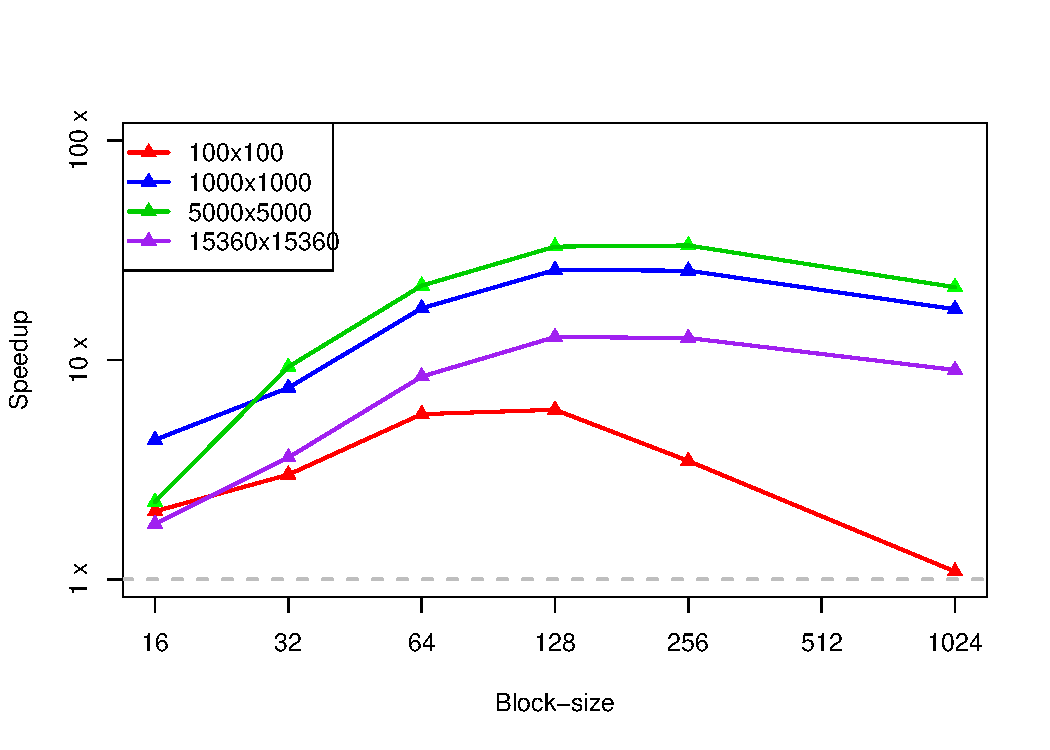
\includegraphics[width=0.75\linewidth]{../plots/fdcalc_shared.pdf}
		\caption{Speedup using shared memory.}
		\label{fig:1}
	\end{subfigure}\hfill
	\begin{subfigure}{0.48\linewidth}
		\centering
		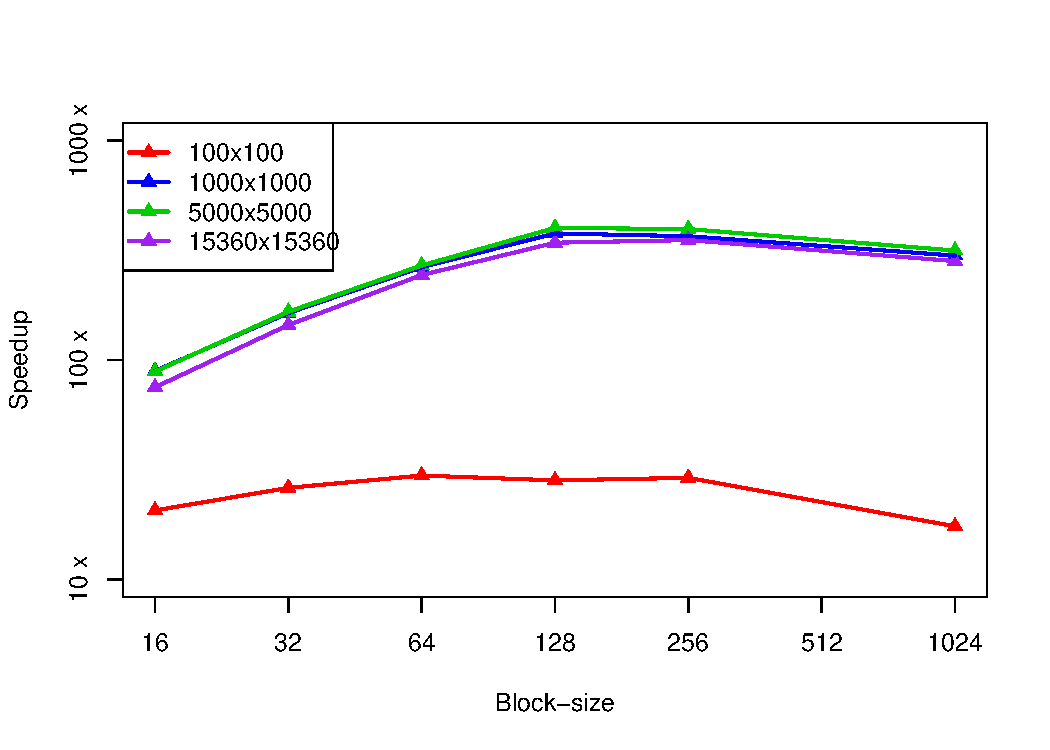
\includegraphics[width=0.75\linewidth]{../plots/fdcalc_glob.pdf}
		\caption{Speedup using global memory.}
		\label{fig:2}
	\end{subfigure}
	\caption{Speedup of calculation times of finite-difference propogation on GPU, using optimisations and using only global memory.}
\end{figure}
\begin{wrapfigure}{l}{0.5\textwidth}
	\centering
	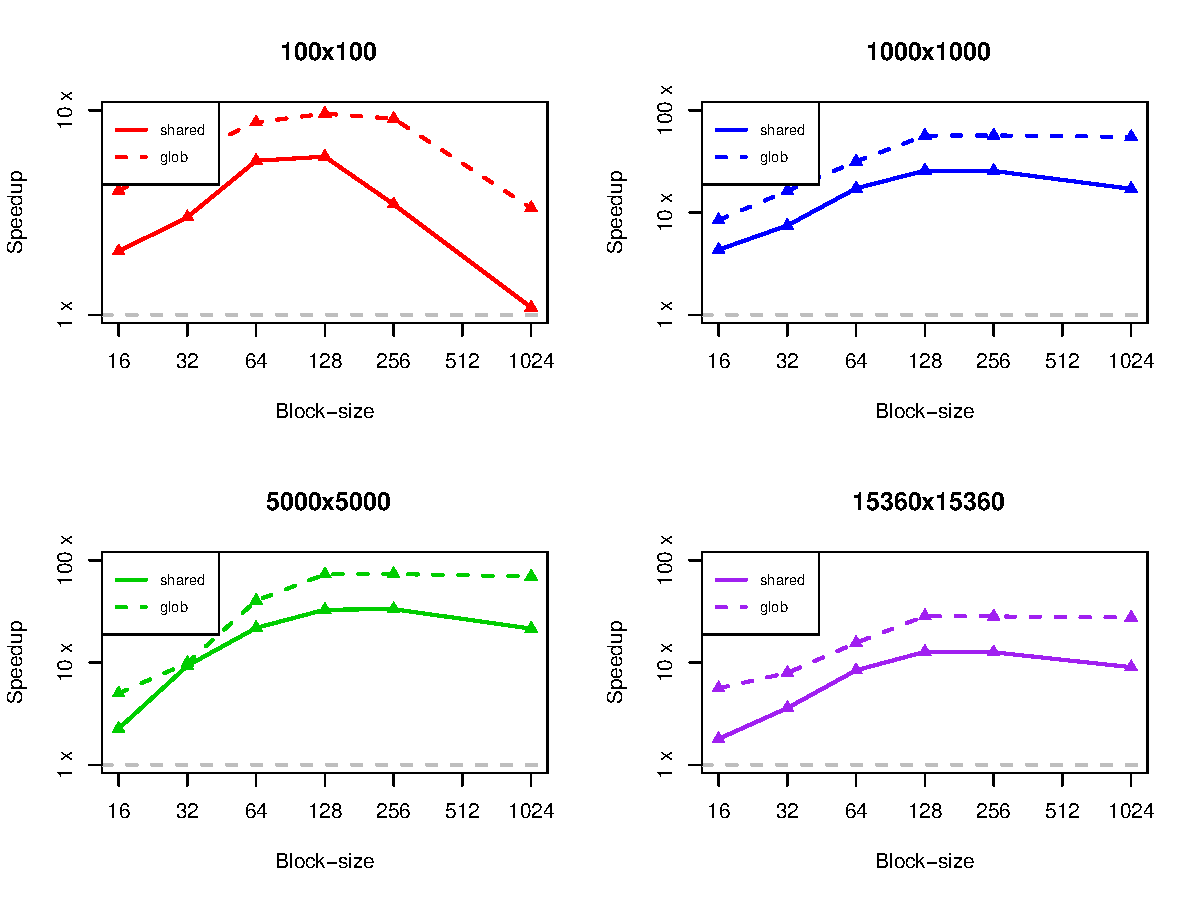
\includegraphics[width=\linewidth]{../plots/fdcalc_sharedvglob.pdf}
	\caption{Speedup of calculation times of finite-difference propogation, comparing global memory and optimisations.}
	\label{fig:3}
\end{wrapfigure}
Figure \ref{fig:1} shows the speedup of the propogation calulation time using the optimised shared memory approach over the CPU's serial time. The speedup reaches up to $\sim453\times$. It increases for the first few increases in matrix size, as expected, however, for $15360\times15360$, there is an evident decrease in speedup. Not clear as to why, it even appears to plateau regarding problem size. Also, interesting to note, there is a clear dip in speedup once the block-size exceeds certain points, depending on the matrix size. For $100\times100$, this is obvious as a block size greater than 128 will be of no benefit to the algorithm, it is not as obvious for the larger matrices but a dip past block-size of $256$ is still seen to a smaller extent. You could extend this to larger block sizes but you would be limited by the max capacity of your shared memory.\\
The difference in this particular case between using shared memory compared to global is arguably negligible here as can bee seen from Figure \ref{fig:3} and \ref{fig:2}. Both methods appear to follow almost the exact same trend.
\subsubsection*{Reduce calculation times}
\begin{figure}
	\centering
	\begin{subfigure}{0.48\linewidth}
		\centering
		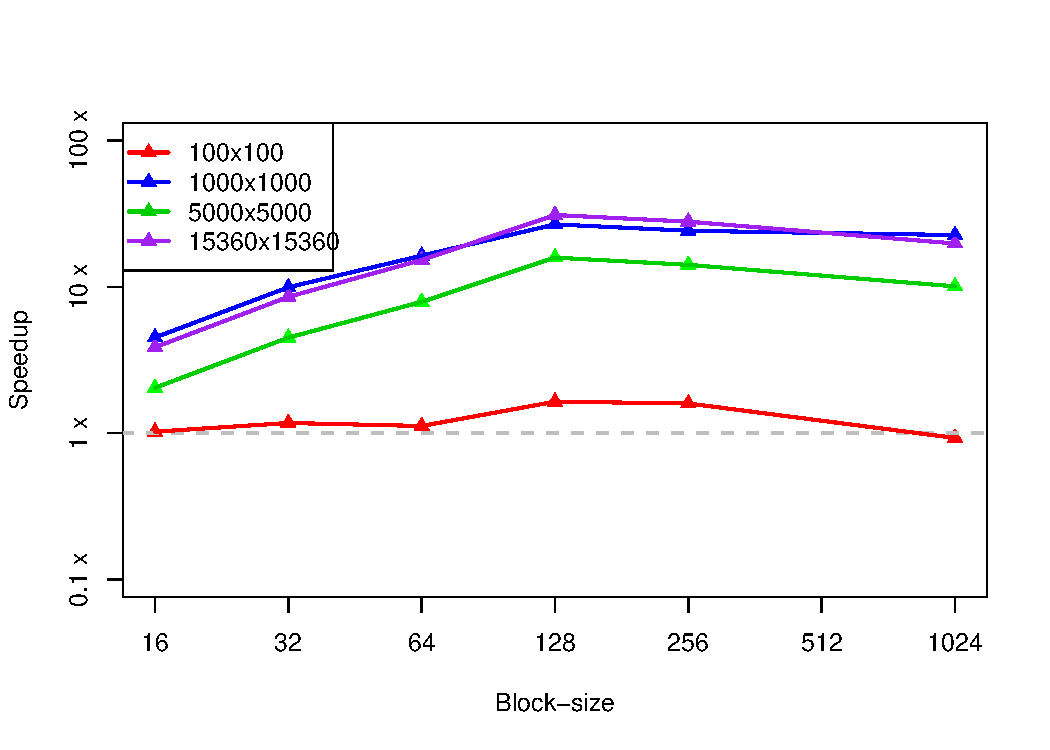
\includegraphics[width=0.85\linewidth]{../plots/redcalc_shared.pdf}
		\caption{Speedup using shared memory.}
		\label{fig:4}
	\end{subfigure}\hfill
	\begin{subfigure}{0.48\linewidth}
		\centering
		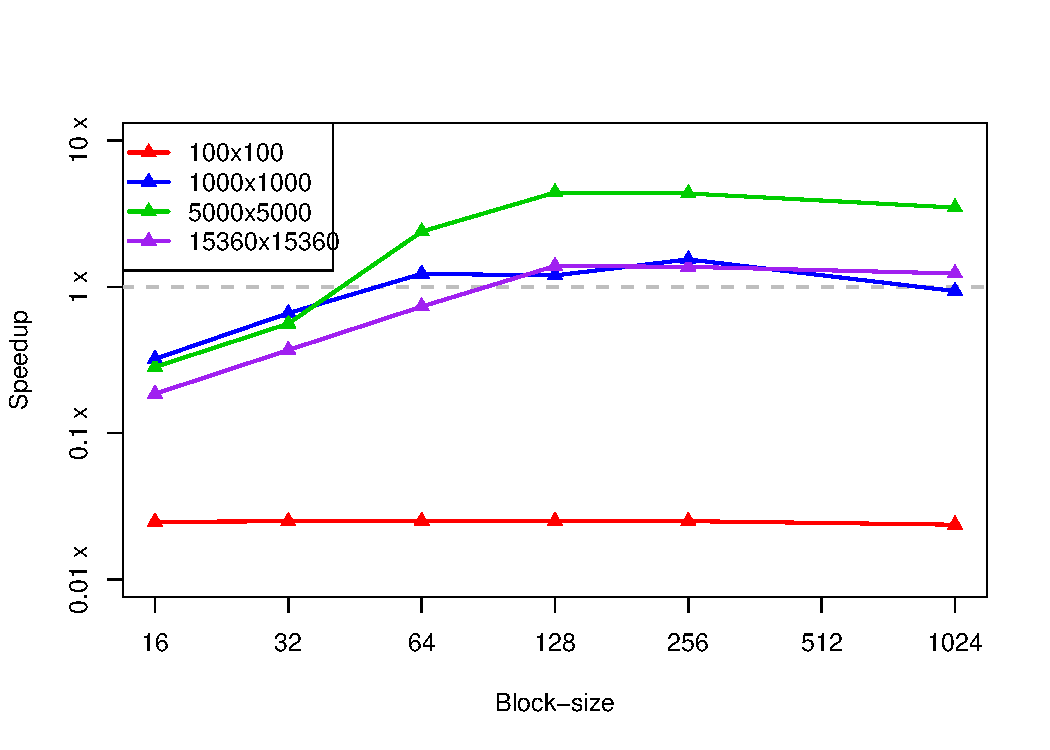
\includegraphics[width=0.85\linewidth]{../plots/redcalc_glob.pdf}
		\caption{Speedup using global memory.}
		\label{fig:5}
	\end{subfigure}
	\caption{Speedup of calculation times of reduce function on GPU, using optimisations and using only global memory.}
\end{figure}
\begin{wrapfigure}{r}{0.5\textwidth}
	\centering
	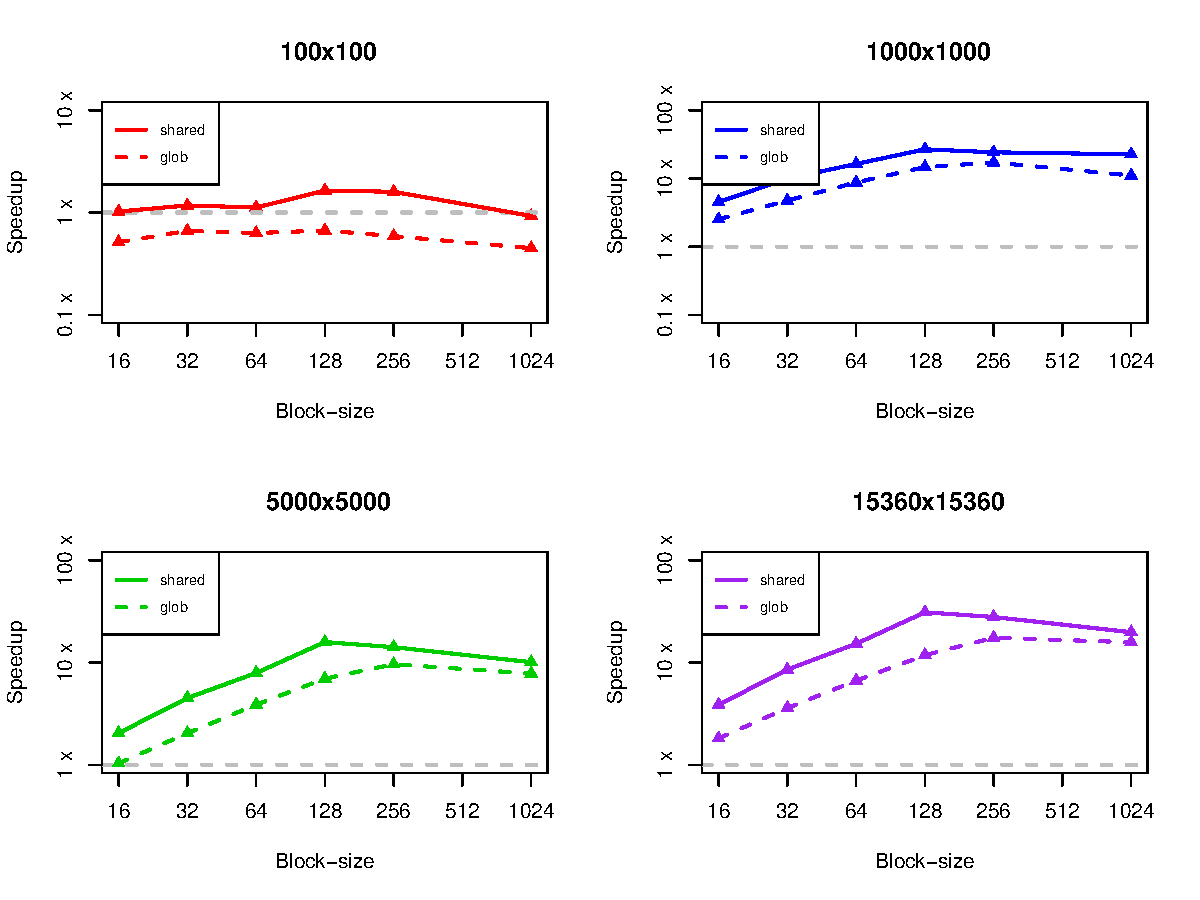
\includegraphics[width=\linewidth]{../plots/red_globvshared.pdf}
	\caption{Speedup of calculation times of reduce function, comparing global memory and optimisations}
	\label{fig:6}
\end{wrapfigure}
The reduce function did not experience the same levels of speedup as seen in the propagation. Presumably due to the increased synchronisation costs of performing the parallelised binary reduction. The results in this case actually started off on par or slower than the serial case, and eventually reach $\sim30\times$ for the $15360\times15360$ matrix and a block size of $128$. The unusual reduction in speedup seen for the larger matrix $15360\times15360$ is not evident in this kernel. These can be seen in Figure \ref{fig:4}.\\
Figure \ref{fig:6} illustrates that the difference in using shared memory versus global which is more obvious here. Expectedly, the shared memory outperforms the global. A dropoff in either case, due to block-size was not as evident in the case of the reduce function. There does appear to be a slight dropoff but not as significant as seen in the propagation. 

\subsubsection*{Allocation \& Device-host transfer times}
\begin{figure}
	\centering
	\begin{subfigure}{0.48\linewidth}
		\centering
		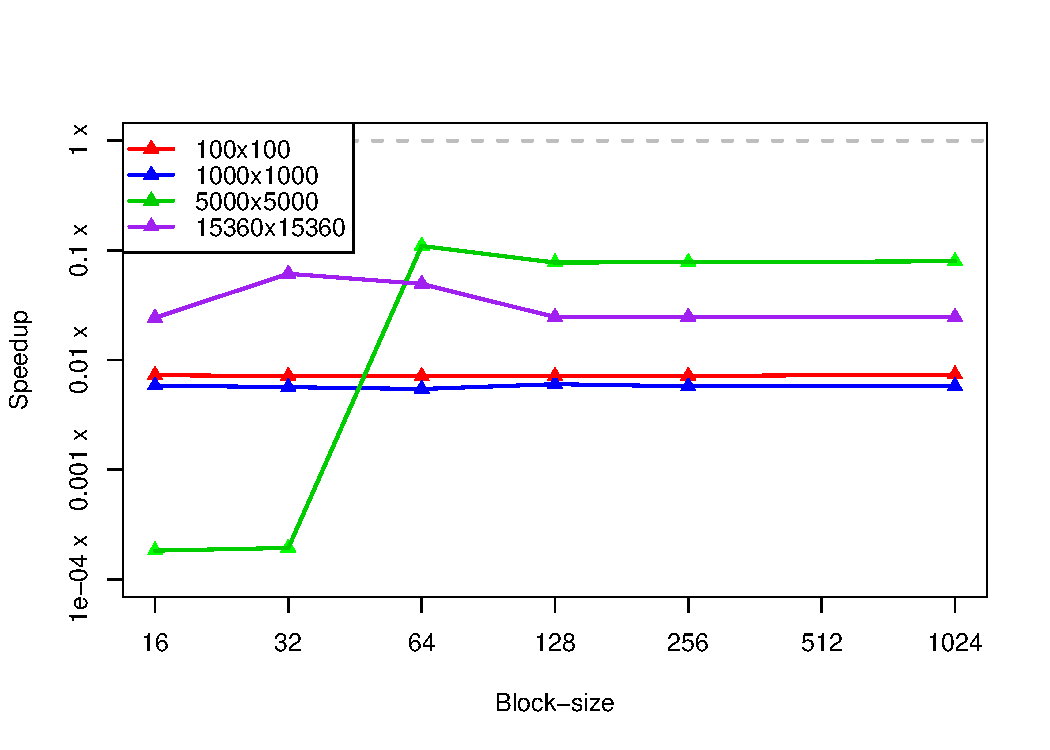
\includegraphics[width=0.85\linewidth]{../plots/alloc_sharedglob.pdf}
		\caption{Speedup of memory allocation time of \texttt{cudaMallocPitch} over \texttt{cudaMalloc}.}
		\label{fig:7}
	\end{subfigure}\hfill
	\begin{subfigure}{0.48\linewidth}
		\centering
		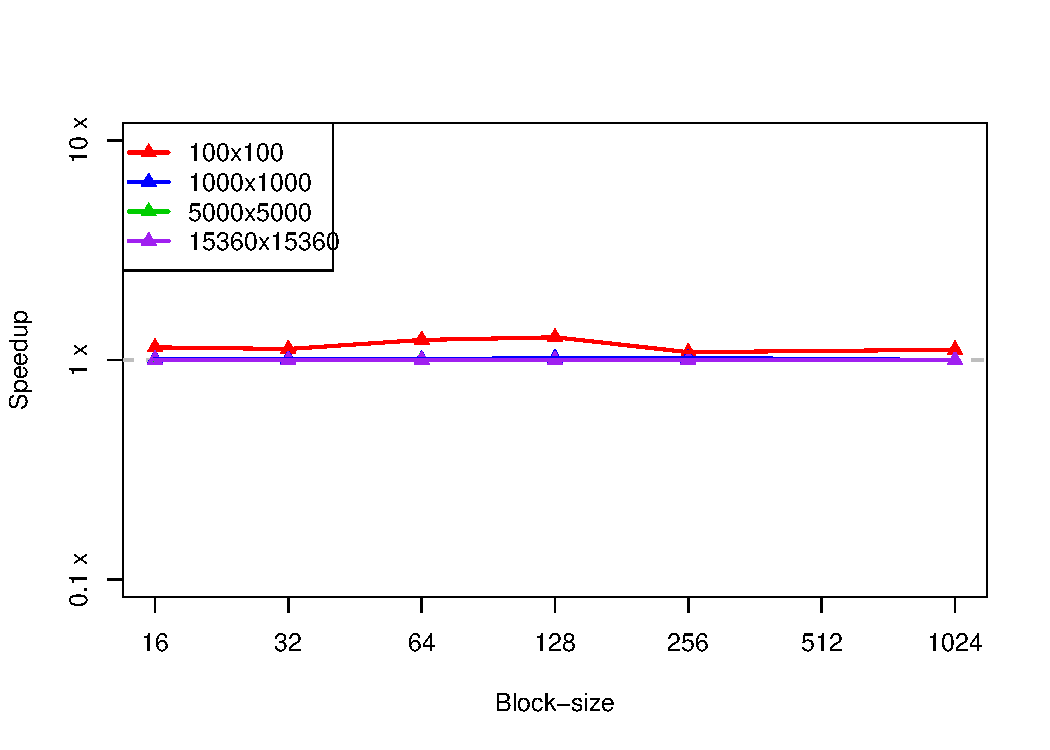
\includegraphics[width=0.85\linewidth]{../plots/RAMsharedglob.pdf}
		\caption{Speedup of device-host transfer time of \texttt{cudaMemcpy2D} over \texttt{cudaMemcpy}.}
		\label{fig:8}
	\end{subfigure}
	\caption{Speedups of allocation time on GPU, and device-host transfer time of \texttt{cudaMallocPitch} and \texttt{cudaMemcpy2D} over \texttt{cudaMalloc} and \texttt{cudaMemcpy}.}
\end{figure}
The allocation time for using \texttt{cudaMalloc} and \texttt{cudaMallocPitch} was tested. Figure \ref{fig:7} would imply that texttt{cudaMalloc} was orders faster, however, in reality it appeared that whatever kernel was ran second in the program actually ran slower. This is contrary to what was seen in the previous assignment where the first kernel was slower and is a result which I cannot come up with justification for.\\
The transfer time from device to host on the other hand was pretty much consistent for both \texttt{cudaMemcpy} and \texttt{cudaMemcpy2D}. No obvious benefits of using 2D data over standard 1D data transfer was seen.
\subsubsection*{SSE}
My SSEs for both optimised and global memory kernels were both reporting $0.00$ for all cases. However, I changed something just before submitting and appeared to cause a bug in my shared memory kernel and so, because of this, I am not reporting accuracy values, as for certain problem/block-sizes the values are incorrect. I did not get the chance to fix this bug.
\pagebreak
\subsubsection*{Total time}
\begin{figure}
	\centering
	\begin{subfigure}{0.48\linewidth}
		\centering
		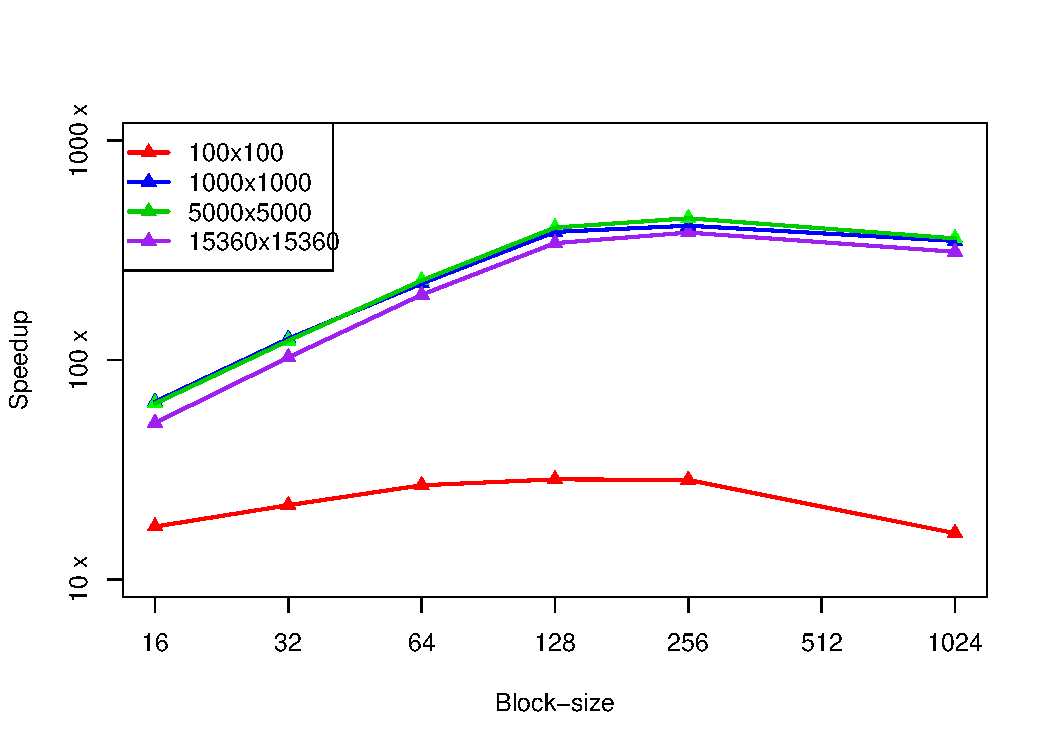
\includegraphics[width=0.85\linewidth]{../plots/tot_shared.pdf}
		\caption{Speedup using shared memory.}
		\label{fig:9}
	\end{subfigure}\hfill
	\begin{subfigure}{0.48\linewidth}
		\centering
		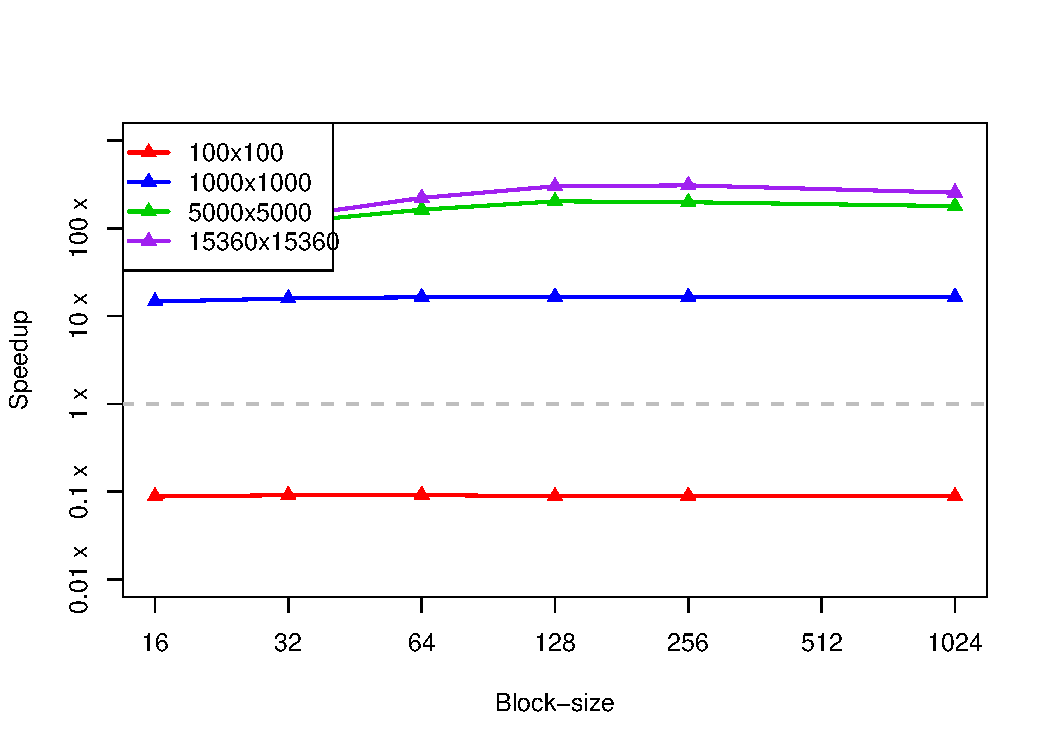
\includegraphics[width=0.85\linewidth]{../plots/tot_glob.pdf}
		\caption{Speedup using global memory.}
		\label{fig:10}
	\end{subfigure}
	\caption{Speedup of total calculation times on GPU, using optimisations and using only global memory.}
\end{figure}
\begin{wrapfigure}{l}{0.5\textwidth}
	\centering
	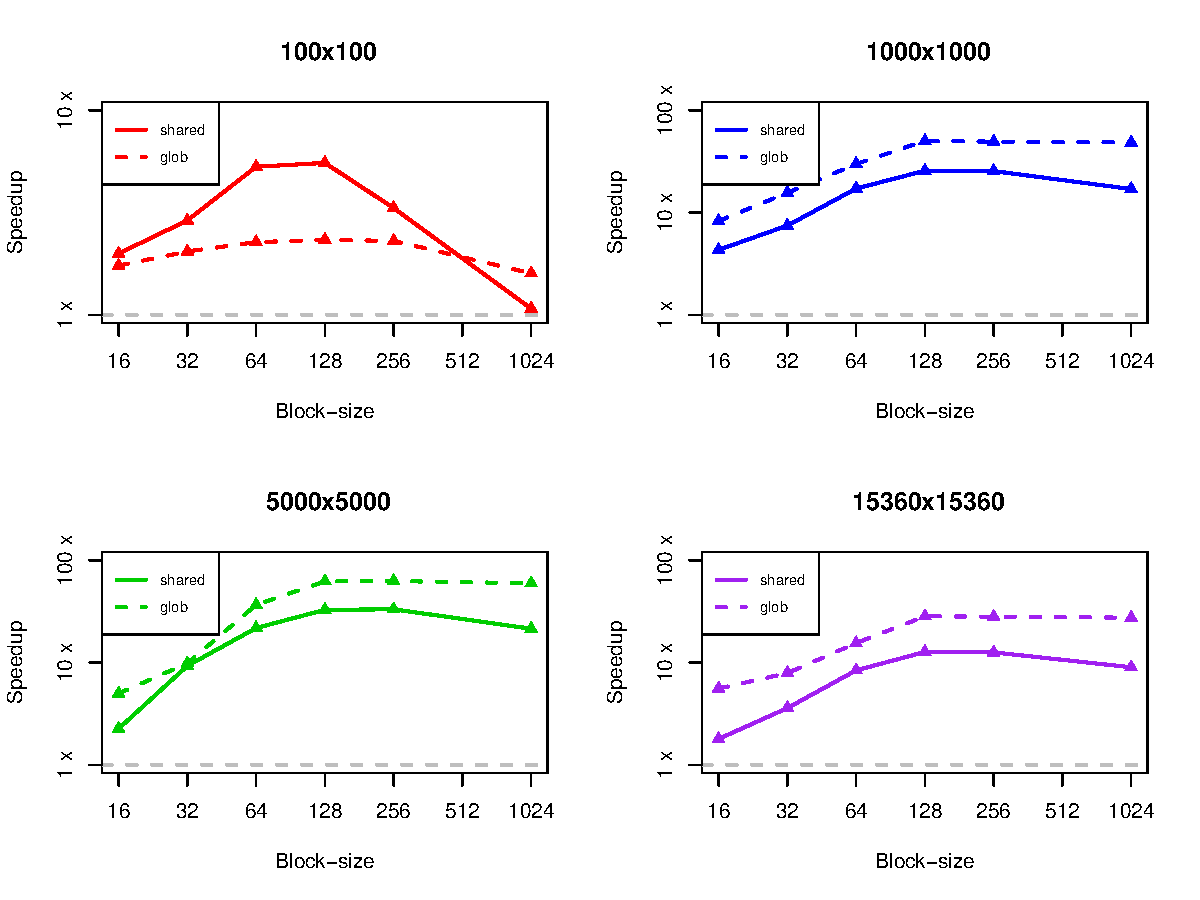
\includegraphics[width=\linewidth]{../plots/tot_globvshared.pdf}
	\caption{Speedup of total calculation time, comparing global memory and optimisations.}
	\label{fig:11}
\end{wrapfigure}
The overall speedups seen are all-in-all, comparable to the results seen in the propagation calculation. An interesting result demonstrating the benefit of using shared memory can be seen in \ref{fig:11}, particularly looking at the $5000\times5000$ case. In this problem, both kernels start off about the same size, but as the block-size grows i.e. the size of the shared memory used, the optimised kernel begins to diverge away and show a more significant speedup while the global memory kernel seems to plateau. Overall speedup reached a max of $\sim442\times$ compared to serial. These results are all illustrared in Figures \ref{fig:9}, \ref{fig:10}. My guess is this is inflated speedups due to poor serial performance.

\subsubsection*{Doubles vs floats}
\begin{figure}
	\centering
	\begin{subfigure}{0.48\linewidth}
		\centering
		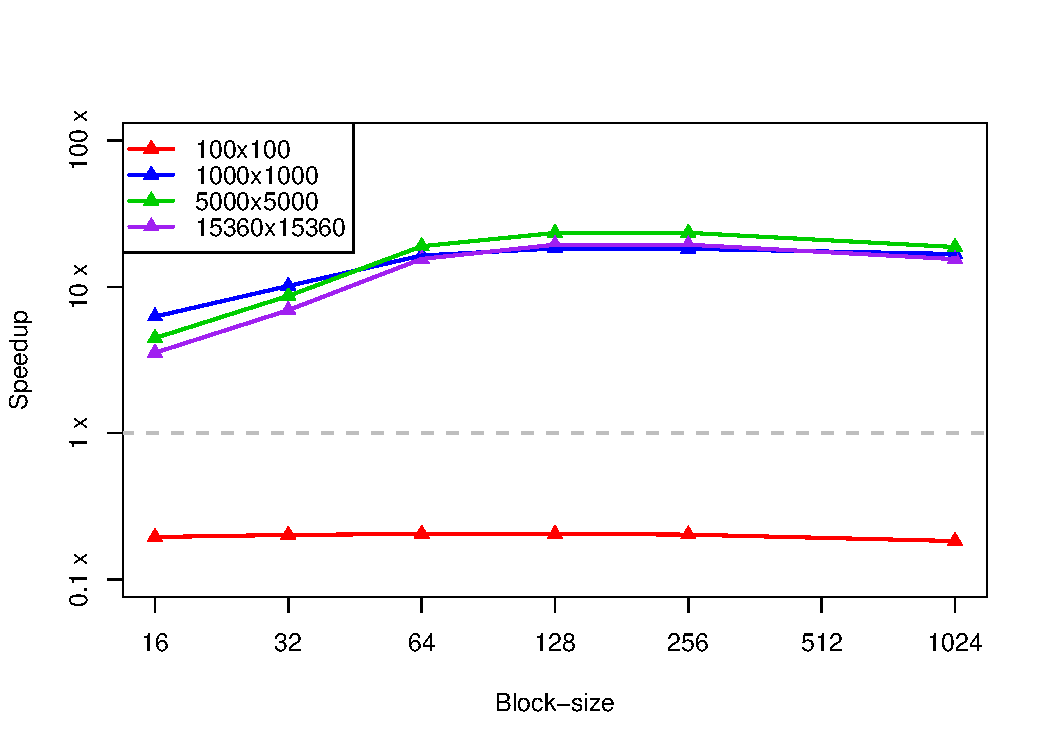
\includegraphics[width=0.85\linewidth]{../plots/tot_double.pdf}
		\caption{Speedup over CPU using double precision numbers.}
		\label{fig:12}
	\end{subfigure}\hfill
	\begin{subfigure}{0.48\linewidth}
		\centering
		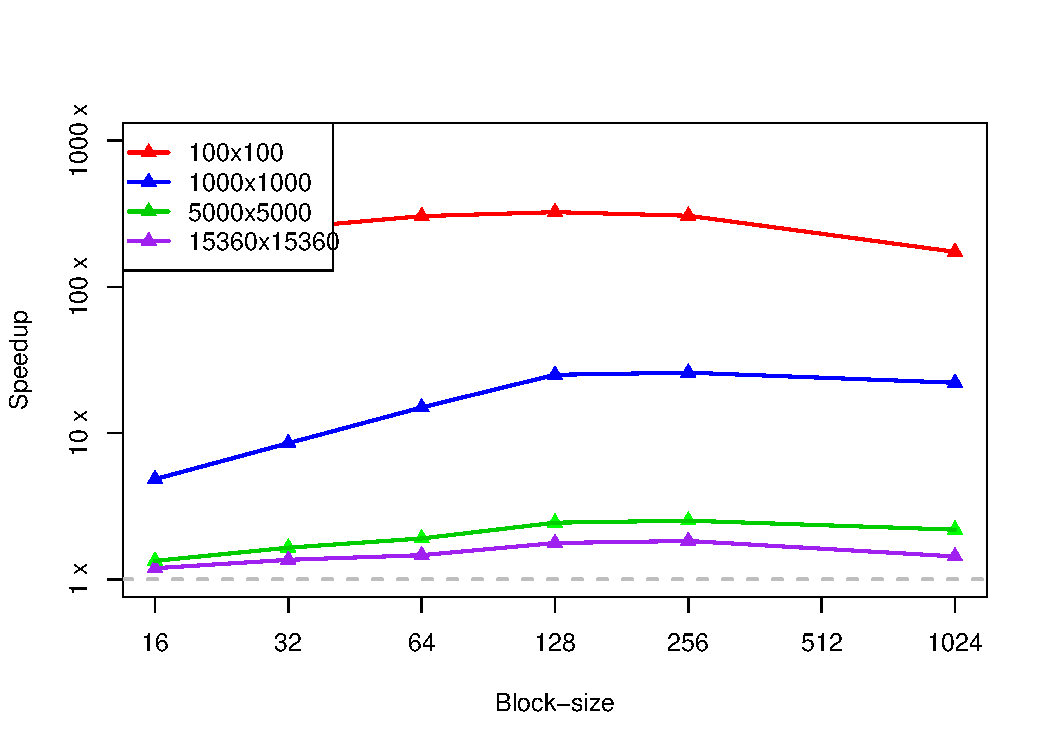
\includegraphics[width=0.85\linewidth]{../plots/tot_doublevfloat.pdf}
		\caption{Speedup of single precision over double precision numbers.}
		\label{fig:13}
	\end{subfigure}
	\caption{Speedup comparisons of floats and doubles.}
\end{figure}
Testing single precision speed versus double precision is shown in Figures \ref{fig:12} and \ref{fig:13}. The speedup over CPU is far more constant in double precision rather interestingly. The single precision values to evidently outperform double precision overall but the speedup reduces by 2 orders as problem size increases, rather strangely.
\end{document}